\subsection*{Zadania na pochodne funkcji różniczkowalnych}
\subsubsection*{Zadanie~9.35.}
\begin{mathfigure*}
    \coordinate (A) at (-3, 0);
    \coordinate (B) at (3, 0);
    \coordinate (C) at (0, 6);
    \coordinate (baseCenter) at (0, 0);
    \coordinate (D) at (-2, 2);
    \coordinate (E) at (2, 2);
    \coordinate (smallBaseCenter) at (0, 2);
    \draw[dashed] (A) -- node[above, near end]{\(R\)} (B);
    \draw (A) -- (C);
    \draw (B) -- (C);
    \draw (baseCenter) ellipse (3 and 0.5);
    \draw[dashed] (C) -- node[right]{\(h\)} (baseCenter);
    \draw[ForestGreen, dashed] (D) -- node[near end, below]{\(r\)} (E);
    \draw[ForestGreen] (D) -- (baseCenter);
    \draw[ForestGreen] (E) -- (baseCenter);
    \draw[ForestGreen] (smallBaseCenter) ellipse (2 and 1/4);
    \path (smallBaseCenter) -- node[left]{\(x\)} (baseCenter);
    \fillpoint*{baseCenter}[\(S\)][below];
    \fillpoint*{smallBaseCenter}[\(T\)][left];
    \fillpoint*{B}[\(B\)][right];
    \fillpoint*{C}[\(C\)][above];
    \fillpoint*{E}[\(E\)][right];
    \drawangle[RoyalBlue, angle radius=0.4cm]{C--B--baseCenter};
    \drawangle[RoyalBlue, angle radius=0.4cm]{C--E--smallBaseCenter};
    \drawrightangle[angle radius=0.4cm]{B--baseCenter--C};
\end{mathfigure*}
Zauważmy, że \(\mangle{CTE} = \mangle{CSB} = 90\degree\) i~\(\mangle{CET} = \mangle{CBS}\). Zatem \(\triangle{TEC} \sim \triangle{SBC}\), czyli
\begin{gather*}
    \frac{r}{R} = \frac{h - x}{h}\\
    r = \frac{R\pars{h - x}}{h}
\end{gather*}
Zdefiniujmy funkcję objętości wewnętrznego stożka w~zależności od jego wysokości \(x\):
\begin{equation*}
    V\pars{x}
        = \frac{1}{3}\pi r^2 \cdot x = \frac{1}{3}\pi \cdot \frac{R^2\pars{h - x}^2 \cdot x}{h^2}
        = \frac{\pi R^2}{3h^2}\pars{h^2x - 2hx^2 + x^3} \qquad x \in \open{0}{h}
\end{equation*}
Obliczmy pochodną tej funkcji:
\begin{gather*}
    V'\pars{x}
        = \frac{\pi R^2}{3h^2}\pars{h^2 - 4hx + 3x^2}
        = \frac{\pi R^2}{3h^2}\pars{3x - h}\pars{x - h}\\
    \upparabola{\frac{h}{3}}{h}
\end{gather*}
Interesuje nas tylko przedział \(\open{0}{h}\). W~przedziale \(\open{0}{\frac{h}{3}}\) pochodna jest dodatnia, dla \(x = \frac{h}{3}\) przyjmuje wartość \(0\), a~w~przedziale \(\open{\frac{h}{3}}{h}\) jest ujemna. Oznacza to, że funkcja \(V\) jest rosnąca w~przedziale \(\open{0}{\frac{h}{3}}\), malejąca w~przedziale \(\open{\frac{h}{3}}{h}\), a~dla \(x = \frac{h}{3}\) przyjmuje lokalną wartość największą:
\begin{equation*}
    V\pars{\frac{h}{3}}
        = \frac{\pi R^2}{3h^2} \cdot \pars{\frac{2h}{3}}^2 \cdot \frac{h}{3}
        = \frac{4\pi R^2h}{81}
\end{equation*}
Zatem optymalna wysokość dla wewnętrznego stożka to \(x = \frac{h}{3}\). Objętość stożka wynosi przy niej \(\frac{4\pi R^2h}{81}\).
\subsubsection*{Zadanie~9.37.}
\begin{mathfigure*}
    \coordinate (S) at (0, 0);
    \coordinate (A) at (-3, -1);
    \coordinate (B) at (1, -1);
    \coordinate (C) at (3, 1);
    \coordinate (D) at (-1, 1);
    \coordinate (E) at (0, 6);
    \coordinate (F) at (-2.18, 0.9);
    \draw (A) -- node[below]{\(a\)} (B) -- (C);
    \draw[dashed] (C) -- (D) -- (A);
    \draw (A) -- (E);
    \draw (B) -- (E);
    \draw (C) -- (E);
    \draw[dashed] (D) -- (E);
    \draw[dashed] (E) -- node[left]{\(h\)} (S);
    \draw (S) -- (A);
    \draw (S) -- node[above, sloped]{\(1\)} (F);
    \fillpoint*{A}[\(A\)][left];
    \fillpoint*{E}[\(E\)][above];
    \fillpoint*{F}[\(F\)][above left];
    \fillpoint*{S}[\(S\)][below];
    \drawrightangle[angle radius=0.4cm]{S--F--E};
    \drawangle[angle radius=0.4cm, RoyalBlue]{S--A--F};
    \drawangle[angle radius=0.4cm, RoyalBlue]{E--S--F};
\end{mathfigure*}
Skoro jest to ostrosłup prawidłowy, to spodek wysokości leży na środku podstawy, zatem \(AS = \frac{a\sqrt{2}}{2}\). Z~twierdzenia Pitagorasa wiemy, \(EF = \sqrt{h^2 - 1}\). Zauważmy, że \(\mangle{EFS} = \mangle{ESA} = 90\degree\) i~\(\mangle{ESF} = \mangle{EAS}\). Zatem \(\triangle{EFS} \sim \triangle{ESA}\), czyli
\begin{gather*}
    \frac{ES}{AS} = \frac{EF}{SF}\\
    \frac{h}{\frac{a\sqrt{2}}{2}} = \frac{\sqrt{h^2 - 1}}{1}\\
    a = \frac{h\sqrt{2}}{\sqrt{h^2 - 1}}
\end{gather*}
Zdefiniujmy funkcję objętości tego ostrosłupa od wysokości \(h\):
\begin{equation*}
    V\pars{h}
        = \frac{1}{3}P_ph
        = \frac{1}{3} \cdot a^2h
        = \frac{1}{3} \cdot \pars{\frac{h\sqrt{2}}{\sqrt{h^2 - 1}}}^2 \cdot h
        = \frac{1}{3} \cdot \frac{2h^3}{h^2 - 1} \qquad h \in \open{1}{+\infty}
\end{equation*}
Obliczmy pochodną tej funkcji:
\begin{equation*}
    V'\pars{h}
        = \frac{1}{3} \cdot \frac{6h^2\pars{h^2 - 1} - 2h^3 \cdot 2h}{\pars{h^2 - 1}^2}
        = \frac{1}{3} \cdot \frac{6h^4 - 6h^2 - 4h^4}{\pars{h^2 - 1}^2}
        = \frac{1}{3} \cdot \frac{2h^4 - 6h^2}{\pars{h^2 - 1}^2}
\end{equation*}
Stała i~mianownik są zawsze dodatnie, więc znak pochodnej zależy tylko od znaku wyrażenia w~liczniku:
\begin{gather*}
    2h^4 - 6h^2\\
    2h^2\pars{h^2 - 3}\\
    2h^2\pars{h + \sqrt{3}}\pars{h - \sqrt{3}}\\
    \upparabola{-\sqrt{3}}{\sqrt{3}}
\end{gather*}
Interesuje nas jedynie przedział \(\open{1}{+\infty}\). W~przedziale \(\open{1}{\sqrt{3}}\) pochodna jest ujemna, dla \(h = \sqrt{3}\) przyjmuje wartość \(0\), a~w~przedziale \(\open{\sqrt{3}}{+\infty}\) jest dodatnia. Oznacza to, że funkcja \(V\) jest malejąca w~przedziale \(\open{1}{\sqrt{3}}\), rosnąca w~przedziale \(\open{\sqrt{3}}{+\infty}\), a~dla \(h = \sqrt{3}\) osiąga globalną wartość najmniejszą:
\begin{equation*}
    V_\p{min} = V\pars{\sqrt{3}} = \frac{1}{3} \cdot \frac{6\sqrt{3}}{3 - 1} = 3\sqrt{3}
\end{equation*}
Zatem najmniejsza możliwa objętość ostrosłupa wynosi \(3\sqrt{3}\) i~jest osiągana przez ostrosłup o~wysokości \(h = \sqrt{3}\).
\subsubsection*{Zadanie~9.41.}
\begin{mathfigure*}
    \coordinate (sphereCenter) at (0, 2);
    \coordinate (A) at (-1.5, 0);
    \coordinate (B) at (1.5, 0);
    \coordinate (C) at (1.5, 4);
    \coordinate (D) at (-1.5, 4);
    \coordinate (E) at (-0.5, 0.45);
    \coordinate (F) at (-0.5, 4.45);
    \coordinate (baseCenter) at (0, 0.2);
    \coordinate (edgeCenter) at (0, 0);
    \draw (sphereCenter) circle[radius=2.5];
    \draw[dotted] (sphereCenter) ellipse (2.5 and 0.5);
    \draw[ForestGreen] (A) -- node[below]{\(a\)} (B) -- (C) -- (D) -- cycle;
    \draw[ForestGreen, dashed] (A) -- (E) -- (B);
    \draw[ForestGreen] (C) -- (F) -- (D);
    \draw[dashed, ForestGreen] (E) -- (F);
    \draw (sphereCenter) -- node[left]{\(\frac{h}{2}\)} (baseCenter);
    \draw (sphereCenter) -- node[above, sloped]{\(R\)} (B);
    \draw[dashed] (baseCenter) -- (B);
    \drawrightangle[angle radius=0.3cm]{B--baseCenter--sphereCenter};
    \fillpoint*{baseCenter}[\(T\)][left];
    \fillpoint*{sphereCenter}[\(S\)][above];
    \fillpoint*{B}[\(B\)][below right];
\end{mathfigure*}
Ponieważ jest to graniastosłup prawidłowy trójkątny, to w~podstawie jest trójkąt równoboczny, a~spodek wysokości znajduje się w~jego środku. Zatem \(TB = \frac{a\sqrt{3}}{3}\). Z~twierdzenia Pitagorasa mamy
\begin{gather*}
    TB^2 + TS^2 = R^2\\
    \pars{\frac{a\sqrt{3}}{3}}^2 + \pars{\frac{h}{2}}^2 = R^2\\
    \frac{a^2}{3} + \frac{h^2}{4} = R^2\\
    h = 2\sqrt{R^2 - \frac{a^2}{3}}
\end{gather*}
Zdefiniujmy funkcję objętości tego graniastosłupa od długości krawędzi jego podstawy \(a\):
\begin{equation*}
    V\pars{a}
        = P_ph
        = \frac{a^2\sqrt{3}}{4} \cdot 2\sqrt{R^2 - \frac{a^2}{3}}
        = \frac{1}{2}\sqrt{3R^2a^4 - a^6} \qquad a \in \open{0}{R\sqrt{3}}
\end{equation*}
Funkcja pierwiastek nie zmienia ekstremów ani monotoniczności funkcji podpierwiastkowej. Podobnie mnożenie przez stałą nie zmienia ekstremów ani monotoniczności mnożonej funkcji. Wystarczy zatem, że zbadamy monotoniczność i~ekstrema funkcji
\begin{equation*}
    W\pars{a}
        = 3R^2a^4 - a^6 \qquad a \in \open{0}{R\sqrt{3}}
\end{equation*}
W~tym celu obliczmy jej pochodną:
\begin{gather*}
    W'\pars{a}
        = 12R^2a^3 - 6a^5
        = 6a^3\pars{2R^2 - a^2}
        = 6a^3\pars{R\sqrt{2} - a}\pars{R\sqrt{2} + a}\\
    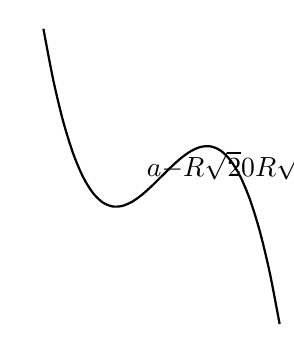
\begin{tikzpicture}
        \drawvec (-2, 0) -- (3, 0) node[below]{\(a\)};
        \draw[domain=-1.5:1.5, smooth, thick] plot (\x, {\x * (1 - \x) * (1 + \x)});
        \fillpoint*{-1, 0}[\(-R\sqrt{2}\)][below left];
        \fillpoint*{0, 0}[\(0\)][above];
        \fillpoint*{1, 0}[\(R\sqrt{2}\)][above right];
    \end{tikzpicture}
\end{gather*}
Interesuje nas tylko przedział \(\open{0}{R\sqrt{3}}\). Pochodna jest dodatnia w~przedziale \(\open{0}{R\sqrt{2}}\), osiąga wartość \(0\) dla \(a = R\sqrt{2}\), a~w~przedziale \(\open{R\sqrt{2}}{R\sqrt{3}}\) jest ujemna. Oznacza to, że funkcja \(W\) jest rosnąca w~przedziale \(\open{0}{R\sqrt{2}}\), malejąca w~przedziale \(\open{R\sqrt{2}}{R\sqrt{3}}\), a~dla \(a = R\sqrt{2}\) osiąga globalną wartość największą. Ponieważ pierwiastek ani stała nie zmieniają ekstremów ani monotoniczności, to samo dotyczy funkcji \(V\). Zatem
\begin{equation*}
    V_\p{max} = V\pars{R\sqrt{2}} = \sqrt{3R^6 - 2R^6} = R^3
\end{equation*}
Maksymalna objętość graniastosłupa wynosi \(R^3\) i~jest osiągana dla \(a = R\sqrt{2}\).
\subsubsection*{Zadanie~9.42.}
\begin{mathfigure*}
    \coordinate (S) at (0, 0);
    \coordinate (A) at (-3, -1);
    \coordinate (B) at (1, -1);
    \coordinate (C) at (3, 1);
    \coordinate (D) at (-1, 1);
    \coordinate (E) at (0, 6);
    \coordinate (edgeCenter) at (-1, -1);
    \coordinate (sphereCenter) at (0, 1.6);
    \coordinate (tangentPoint) at (-0.69, 1.15);
    \draw (A) -- (B) -- node[below right]{\(a\)} (C);
    \draw[dashed] (C) -- (D) -- (A);
    \draw[ForestGreen] (sphereCenter) circle[radius=1.6];
    \draw[ForestGreen, dashed] (sphereCenter) ellipse (1.6 and 0.5);
    \draw (A) -- (E);
    \draw (B) -- (E);
    \draw (C) -- (E);
    \draw[dashed] (D) -- (E);
    \draw[dashed, Orange] (E) -- node[right]{\(h\)} (S);
    \draw (S) -- (edgeCenter) -- (E);
    \draw[densely dotted, thick] (sphereCenter) -- node[right]{\(R\)} (S);
    \fillpoint*{A}[\(A\)][left];
    \fillpoint*{E}[\(E\)][above];
    \fillpoint*{S}[\(S\)][below];
    \fillpoint*{edgeCenter}[\(P\)][below];
    \fillpoint*{1.6, 1.6};
    \fillpoint*{-1.6, 1.6};
    \fillpoint*{sphereCenter}[\(T\)][right];
    \draw (sphereCenter) -- node[below, sloped]{\(R\)} (tangentPoint);
    \fillpoint*{tangentPoint}[\(K\)][left];
    \drawangle[angle radius=0.4cm, RoyalBlue]{sphereCenter--tangentPoint--E};
    \drawangle[angle radius=0.4cm, RoyalBlue]{S--edgeCenter--E};
    \drawrightangle[angle radius=0.3cm]{E--S--edgeCenter};
    \drawrightangle[angle radius=0.3cm]{E--sphereCenter--tangentPoint};
\end{mathfigure*}
Ponieważ jest to ostrosłup prawidłowy czworokątny, to w~podstawie jest kwadrat, a~jego środek to spodek wysokości ostrosłupa. Oznacza to, że \(PS = \frac{a}{2}\). Zauważmy, że \(\mangle{ETK} = \mangle{ESP} = 90\degree\) i~\(\mangle{EKT} = \mangle{EPS}\). Zatem \(\triangle{ETK} \sim \triangle{ESP}\), czyli
\begin{gather*}
    \frac{ET}{ES} = \frac{TK}{SP}\\
    \frac{h - R}{h} = \frac{R}{\frac{a}{2}}\\
    a = \frac{2Rh}{h - R}
\end{gather*}
Zdefiniujmy funkcję objętości ostrosłupa w~zależności od jego wysokości:
\begin{equation*}
    V\pars{h}
        = \frac{1}{3}P_ph
        = \frac{1}{3} \cdot a^2h
        = \frac{1}{3} \cdot \pars{\frac{2Rh}{h - R}}^2 \cdot h
        = \frac{1}{3} \cdot \frac{4R^2h^3}{h^2 - 2Rh + R^2} \qquad h \in \open{2R}{+\infty}
\end{equation*}
Obliczmy pochodną tej funkcji:
\begin{equation*}
    \begin{split}
        V'\pars{h}
            &= \frac{1}{3} \cdot \frac{12R^2h^2\pars{h^2 - 2Rh + R^2} - \pars{2h - 2R} \cdot 4R^2h^3}{\pars{h - R}^4}
            = \frac{1}{3} \cdot \frac{12R^2h^4 - 24R^3h^3 + 12R^4h^2 - 8R^2h^4 + 8R^3h^3}{\pars{h - R}^4}\\
            &= \frac{1}{3} \cdot \frac{4R^2h^4 - 16R^3h^3 + 12R^4h^2}{\pars{h - R}^4}
    \end{split}
\end{equation*}
Stała i~mianownik są zawsze dodatnie, więc znak pochodnej zależy jedynie od wyrażenia w~liczniku ułamka:
\begin{gather*}
    4R^2h^4 - 16R^3h^3 + 12R^4h^2\\
    4R^2h^2\pars{h^2 - 4Rh + 3R^2}\\
    4R^2h^2\pars{h - R}\pars{h - 3R}\\
    \begin{tikzpicture}
        \drawvec (-1, 0) -- (4, 0) node[below]{\(h\)};
        \draw[domain=-1:3.2, smooth, thick] plot (\x, {0.5 * \x * \x * (\x - 1) * (\x - 3)});
        \fillpoint*{0, 0}[\(0\)][below];
        \fillpoint*{1, 0}[\(R\)][above right];
        \fillpoint*{3, 0}[\(3R\)][below right];
    \end{tikzpicture}
\end{gather*}
Interesuje nas tylko przedział \(\open{2R}{+\infty}\). W~przedziale \(\open{2R}{3R}\) pochodna jest ujemna, dla \(h = 3R\) przyjmuje wartość \(0\), a~w~przedziale \(\open{3R}{+\infty}\) jest dodatnia. Oznacza to, że w~przedziale \(\open{2R}{3R}\) funkcja \(V\) jest malejąca, w~przedziale \(\open{3R}{+\infty}\) jest rosnąca, a~dla \(h = 3R\) przyjmuje globalną wartość najmniejszą:
\begin{equation*}
    V\pars{3R}
        = \frac{1}{3} \cdot \frac{4R^2 \cdot 27R^3}{9R^2 - 6R^2 + R^2}
        = 9R^3
\end{equation*}
Ostrosłup o~najmniejszej objętości równej \(9R^3\) posiada wysokość \(h = 3R\).
